\documentclass[../homework.tex]{subfiles}

\pagestyle{fancy}
\fancyhf{}
\rhead{Hanzhi Zhou}
\lhead{Physics 2415 Homework}
\cfoot{\thepage}

\begin{document}
\subsection{Problem 2.2}
\subsubsection*{a)}

\paragraph{i)}
\begin{subp}

	First calculate the charge as a function of radius for $r \le r_0$
	\begin{equation*}
		Q(r) = \int\rho~dV = \int_{0}^{r} \frac{C}{r'} 4 \pi r'^2 dr' = 4 C \pi \int_{0}^{r} r' dr' = 4\pi C \frac{1}{2} r^2 = 2 \pi C r^2
	\end{equation*}

	For $r \le r_0$
	\begin{align*}
		\Phi(r) & = \frac{Q}{\epsilon_0} = \frac{2 \pi C r^2}{\epsilon_0} = E(r) \times 4 \pi r^2 \\
		E(r)    & = \frac{C}{2 \epsilon_0}
	\end{align*}

	For $r > r_0$
	\begin{align*}
		\Phi(r) & = \frac{Q}{\epsilon_0} = \frac{2\pi C r_0^2}{\epsilon_0} = E(r) \times 4 \pi r^2 \\
		E(r)    & = \frac{Cr_0^2}{2 \epsilon_0 r^2}
	\end{align*}
\end{subp}

\paragraph{ii)}
\begin{subp}
	
	For $r > r_0$
	\begin{align*}
		V(r) = -\frac{C r_0^2}{2\epsilon_0} \int_{\infty}^{r} \frac{1}{r'^2} dr' = \frac{C r_0^2}{2\epsilon_0}\frac{1}{r}
	\end{align*}

	For $r \le r_0$
	\begin{align*}
		V(r) & = V(r_0) - \int_{r_0}^{r} \frac{C}{2\epsilon_0} dr'                      \\
		     & = \frac{C r_0}{2\epsilon_0} - \frac{C}{2 \epsilon_0}\left[r - r_0\right] \\
		     & = \frac{C}{\epsilon_0} \left(r_0-\frac{r}{2}\right)
	\end{align*}
\end{subp}

\paragraph{iii)}
\begin{subp}
	\begin{figure}[H]
		\centering
		\begin{subfigure}{.4\textwidth}
			\centering
			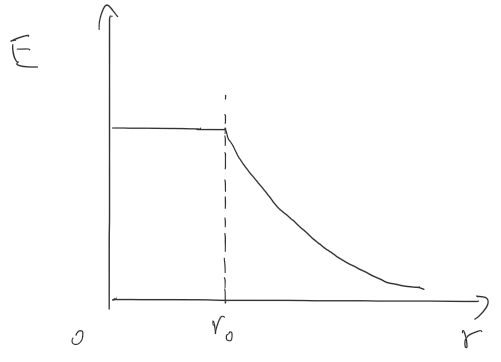
\includegraphics[width=\linewidth]{p2-a-sketch-E.png}
		\end{subfigure}%
		\begin{subfigure}{.4\textwidth}
			\centering
			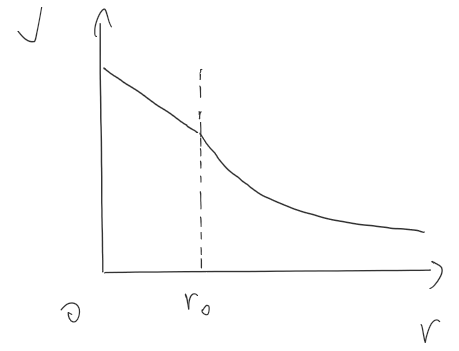
\includegraphics[width=\linewidth]{p2-a-sketch-V.png}
		\end{subfigure}
	\end{figure}
\end{subp}

\subsubsection*{b)}
\paragraph{i)}

\begin{subp}

	First find the charge enclosed as a function of radius. \\

	% Let $Q_1$, $V_1$ to be the charge and the volume of the inner sphere, and let $Q_2$, $V_2$ to be the charge and the volume of the outer shell, respectively.

	For $r < a$, $Q(r) = 0$, because charges reside on the surface of a conductor. 
	%% 
	% \begin{equation*}
	% 	Q(r) = \rho V(r) = \frac{Q_1}{V_0} V(r) = \frac{Q_1}{\frac{4}{3}\pi a^3} \frac{4}{3} \pi r^3  = \frac{Q_1}{a^3} r^3
	% \end{equation*}

	For $a < r < b$, $Q(r) = +2Q$.\\

	For $b < r < c$, $Q(r) = 0$, because the $+2Q$ inside attracts $-2Q$ charges on the inner surface of the conducting shell, and the net charge enclosed is zero. \\
	% \begin{equation*}
	% 	Q(r) = Q_1 + \frac{Q_2}{V_2} V(r) = Q_1 + \frac{Q_2}{\frac{4}{3} \pi (c^3 - b^3)} \frac{4}{3} \pi (r^3 - b^3) = Q_1 + \frac{Q_2}{(c^3 - b^3)} (r^3 - b^3)
	% \end{equation*}

	For $r > c$, $Q(r) = +Q$. \\

	Then, use Gauss's law to find the electric field
	\begin{align*}
		\Phi(r) &= \frac{Q(r)}{\epsilon_0} = E(r)~4\pi r^2 \\
		E(r) &= \frac{Q(r)}{4 \pi \epsilon_0 r^2} 
		% \frac{Q} {4\pi\epsilon_0} \frac{r}{a^3}
	\end{align*}

	For $r < a$, 
	\begin{equation*}
		E(r) = \frac{0}{4 \pi \epsilon_0 r^2} = 0
	\end{equation*}

	For $a < r < b$, 
	\begin{equation*}
		E(r) = \frac{2Q}{4 \pi \epsilon_0 r^2} = \frac{Q}{2\pi \epsilon_0 r^2}
	\end{equation*}

	For $b < r < c$, 
	\begin{equation*}
		E(r) = \frac{0}{4 \pi \epsilon_0 r^2} = 0
	\end{equation*}

	For $r > c$,
	\begin{equation*}
		E(r) = \frac{Q}{4 \pi \epsilon_0 r^2} 
	\end{equation*}
\end{subp}

\paragraph{ii)}
\begin{subp}

	-2Q amount of charges appear on the inner surface of the shell. +Q amount of charges appear on the outer surface of the shell.
\end{subp}

\paragraph{iii)}
\begin{subp}
	\begin{figure}[H]
		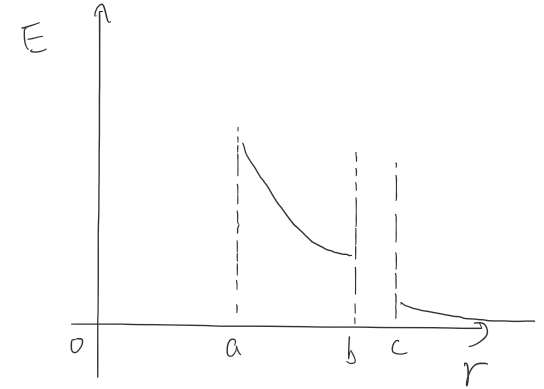
\includegraphics[width=.6\linewidth]{p2-b-sketch.png}
	\end{figure}
\end{subp}
\end{document}